\documentclass{article}
%% Useful packages
\usepackage[utf8]{inputenc}
\usepackage[a4paper,left=2cm,right=2cm,top=2cm,bottom=2cm]{geometry}
\usepackage{crop,graphicx,amsmath,array,color,amssymb,fancyhdr,lineno}
\usepackage{flushend,stfloats,amsthm,chngpage,times,,lipsum,lastpage} 
\usepackage{calc,listings,color,wrapfig,tabularx,longtable,enumitem}
\usepackage[style=numeric-comp,backend=biber]{biblatex}
\addbibresource{Refs.bib}
\usepackage{lineno}
%%%%%%%%%%%%   Header and Footer  %%%%%%%%%%%%%
\pagestyle{fancy}
\fancypagestyle{plain}{%
  \renewcommand{\headrulewidth}{0pt}%
  \fancyhf{}%
}

\title{%
  Project Title \\
  \large Subtitle}
\author{Clément}
%%%%%%%%%%%%   tiltle  %%%%%%%%%%%%%
\begin{document}

\begin{titlepage}

    \newcommand{\HRule}{\rule{\linewidth}{0.5mm}} % Defines a new command for the horizontal lines, change thickness here
    
    %----------------------------------------------------------------------------------------
    %	LOGO SECTION
    %----------------------------------------------------------------------------------------
    \center
    \includegraphics[width=5cm]{logo_nantes.png}\\[1cm] % Include a department/university logo - this will require the graphicx package
     
    %----------------------------------------------------------------------------------------
    
    \center % Center everything on the page
    
    %----------------------------------------------------------------------------------------
    %	HEADING SECTIONS
    %----------------------------------------------------------------------------------------
    
    
    \textsc{\LARGE Nantes Université - M2 (MACS)  }\\[1.5cm] % Name of your university/college
    
    \vspace{1cm}
    
    \textsc{\Large \textbf{Calcul scientifique numérique} }\\[0.5cm] % Major heading such as course name
    \textsc{\large  Language C}\\[0.5cm] % Minor heading such as course title
    
    %----------------------------------------------------------------------------------------
    %	TITLE SECTION
    %----------------------------------------------------------------------------------------
    
    \vspace{2cm} 
    
    \makeatletter
    \HRule \\[0.4cm]
    { \huge \bfseries Projet 1}\\[0.4cm] % Title of your document
    \HRule \\[1.5cm]
     
    %----------------------------------------------------------------------------------------
    %	AUTHOR SECTION
    %----------------------------------------------------------------------------------------
    
    \begin{minipage}{0.4\textwidth}
    \begin{flushleft} \large
    \emph{Etudiant}\\
     \textbf{MARIOT} Clement % Your name
    \\[1.2em]
    \emph{ID No:}\\
    00000 \\[1.2em]
    \end{flushleft}
    \end{minipage}
    ~
    \begin{minipage}{0.4\textwidth}
    \begin{flushright} \large
    \emph{Enseignant} \\
    Dr \textbf{NACHAOUI} Abdeljalil  \\[1.2em] % Supervisor's Name
    \end{flushright}
    \end{minipage}\\[2cm]
    \makeatother
    
    % If you don't want a supervisor, uncomment the two lines below and remove the section above
    %\Large \emph{Author:}\\
    %John \textsc{Smith}\\[3cm] % Your name
    
    %----------------------------------------------------------------------------------------
    %	DATE SECTION
    %----------------------------------------------------------------------------------------
    
    {\large \today}\\[2cm] % Date, change the \today to a set date if you want to be precise
    
    \vfill % Fill the rest of the page with whitespace
    
    \end{titlepage}
\sffamily
\fancyhf{}
\fancyhead[L]{Compte Rendu}
\fancyhead[R]{}
\fancyfoot[R]{ \bf\thepage\ \rm }%
%%%%%%%%%%%%   Htitle  %%%%%%%%%%%%%
\newpage
%%%%%%%%%%%%  table of contente  %%%%%%%%%%%%%
\tableofcontents
%%%%%%%%%%%%  section 1   %%%%%%%%%%%%%
\newpage


\section{Présentation du problème}


On considère un problème géométrique inverse où une partie inconnue de la frontière du domaine est construite à partir de conditions limites surdéterminées. Ainsi pour résoudre ce problème de Cauchy pour les équations de Laplace, on utilisera la série de Fourrier pour formuler une équation intégrale de Fredholm de premier type. Puis par une méthode de régularisation, on récupère une équation intégrale de Fredholm de second type résolvable. Enfin, les coordonnées de la partie inconnue de la frontière sont ensuite obtenues sous forme de racines d’équations non linéaires en utilisant une méthode de type Newton. 

Ainsi soit $\Omega \subset R^2$, le problème est posé comme suit : 

            Trouver $T$ et $\Gamma \subset \delta \Omega$ tels que,
\begin{equation}
  \label{eq/pb1}
  \left\{
    \begin{array}{rcl}
      \Delta T = 0 && \textrm{dans $\Omega$,}\\
      \frac{\delta T}{\delta x} = 0 && \textrm{sur $\Gamma_1 \cup \Gamma_2$,}\\
      T = T_0 && \textrm{sur $\Gamma$,}\\
      -\frac{\delta T}{\delta y}(x, 0) = q_0(x) && \textrm{sur $\Gamma_0$,}\\
      T(x, 0) = f_0(x) && \textrm{sur $\Gamma_0$,}
    \end{array}
  \right.
  \tag{P1}
\end{equation}
Où $\delta \Omega = \Gamma_0 \cap \Gamma_1 \cap \Gamma_2 \cap \Gamma$
$\Gamma$ est la courbe définie par $\Gamma = (x, f(x))$ avec $x \in \Gamma_0$

\begin{figure}[h]
  \centering
  \includegraphics[width=7cm]{domaine1.png}
  \label{fig/domaine}
  \caption{Le domaine $\Omega$}
\end{figure}

\vspace{0.5cm}

Considérons maintenant $D$, un rectangle tel que $\Omega \subset D$ . On note $\tilde{\Gamma_1}$ le prolongement de $\Gamma_1$ et $\tilde{\Gamma_2}$ celui de de $\Gamma_2$ tel que :
\begin{equation}
    \delta D = \Gamma_0 \cup \tilde{\Gamma_1} \cup \tilde{\Gamma_2} \cup \Gamma_3
\end{equation}
On s'interesse à la condition aux limites sur $\Gamma_3$ :
\begin{equation}
    \tilde{T}(x, H) = f_3(x) 
\end{equation}
Ainsi le problème définit sur $D$ est :
            Trouver $\tilde{T}$ tel que,
\begin{equation}
  \label{eq/P2}
  \left\{
    \begin{array}{rcl}
      \Delta \tilde{T} = 0 && \textrm{dans $D$,}\\
      \frac{\delta \tilde{T}}{\delta x} = 0 && \textrm{sur $\tilde{\Gamma_1} \cup \tilde{\Gamma_2}$,}\\
      \tilde{T}(x, H) = f_3(x) && \textrm{sur $\Gamma_3$,}\\
      -\frac{\delta \tilde{T}}{\delta y}(x, 0) = q_0(x) && \textrm{sur $\Gamma_0$,}\\
      \tilde{T}(x, 0) = f_0(x) && \textrm{sur $\Gamma_0$,}
    \end{array}
  \right.
  \tag{P2}
\end{equation}



avec la donnée $f_3(x)$ inconnue et doit être reconstruite.

On va résoudre ce problème en deux étapes, on commence par résoudre le problème de Cauchy linéaire (P2) sur un domaine fixe $D$. Puis on résolve un système non linéaire pour déterminer la frontière $\Gamma$ de la forme :
\begin{equation}
    T^\alpha(x,y) - T_0(x) = 0
\end{equation}


\section{Détermination des fonctions sur le bord}
On choisi pour la suite comme solution exacte :
\begin{equation}
    T_{exacte}(x, y) = cosh(\pi y)cos(\pi x)
\end{equation}
Car la solution proposée dans l'énoncé du projet ne respecte pas les conditions limtes appliquées en $\tilde{\Gamma_1} \cup \tilde{\Gamma_2}$
Ainsi on détermine $f_0$, $q_0$ et $f_3$ à l'aide de (P2):
\begin{equation}
    f_0(x) = T_{exacte}(x, 0) = cos(\pi x)
\end{equation}
\begin{equation}
    q_0(x) = -\frac{\delta T}{\delta y}(x, 0) = -\pi sinh(0\pi)cos(\pi x) = 0
\end{equation}
\begin{equation}
    f_3(x) = T_{exacte}(x, H) = cosh(\pi H)cos(\pi x)
\end{equation}


\section{Choix du coefficient de Lavrentier}
Pour commence suite probablement à une erreur je remarque que la quantité $||T_{ex} - T_{cal}||_{L^2(\Gamma_3)}$ augmentait lorsque le coefficient $\alpha$ s'approchait de $0$. J'ai pensé à un bug ou une faute de calcul mais malgré avoir épluché les logs du programme je n'ai rien trouvé. Je pense que je travail en fait sur $\frac{1}{\alpha}$ et donc on étudie $||T_{ex} - T_{cal}||_{L^2(\Gamma_3)}$ pour $\alpha \in [5, 100]$. On a choisit cet intervalle car celui proposé dans l'énoncé donne des erreurs bien trop élévée par rapport à ce que l'on peut avoir sur l'intervalle choisit. On obtient ainsi la figure suivante :


\begin{figure}[h]
  \centering
  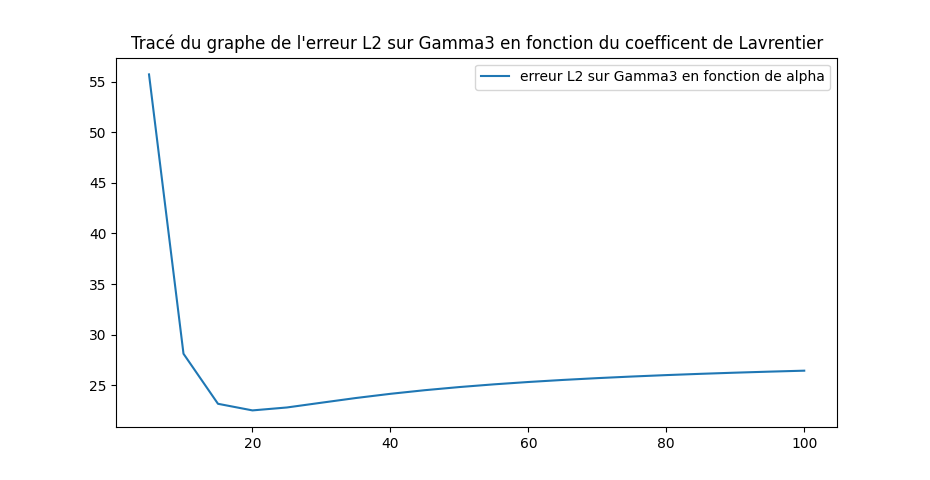
\includegraphics[width=10cm]{erreur_sur_Gamma3_lavrentier.png}
  \label{fig/domaine}
  \caption{$||T_{ex} - T_{cal}||_{L^2(\Gamma_3)}$ en fonction de $\alpha$}
\end{figure}

\vspace{1cm}
Cette figure a été tracée avec une discrétisation de cent points sur le segment $\Gamma_3$, et avec $H = L = 1$ ainsi qu'une approximation de toutes les séries utilisées par la somme de leurs  vingt premiers termes. On remarque que pour ces paramètres le $\alpha$ optimal est $\alpha = 20$ que l'on fixera dans la suite de ce projet.

\newpage

\section{Affichage des fonctions}
On utilise le language python pour afficher nos figures. Pour cela on a crée un maillage régulier de $10 \times 10$
sur $\Omega$.

\begin{figure}[h]
  \centering
  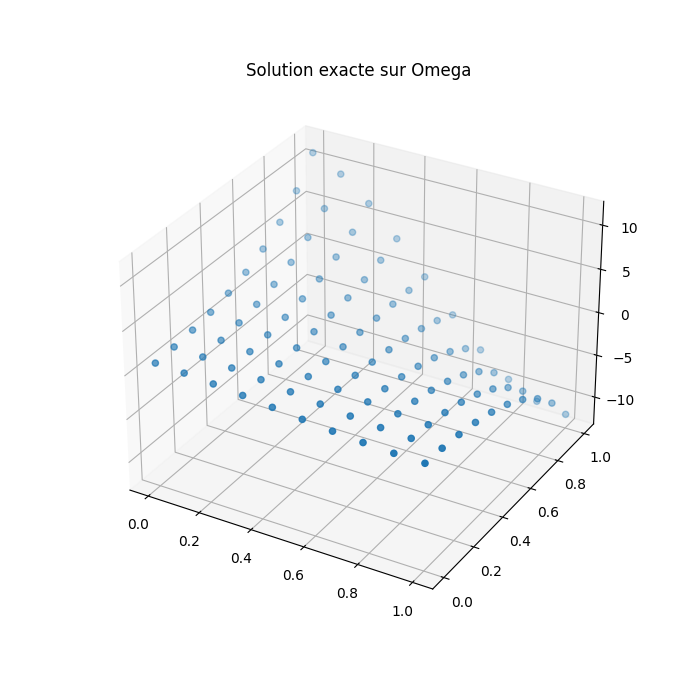
\includegraphics[width=7cm]{solex_omega.png}
  \label{fig/domaine}
  \caption{La solution exacte sur le maillage de $\Omega$}
\end{figure}

\vspace{1cm}

\begin{figure}[h]
  \centering
  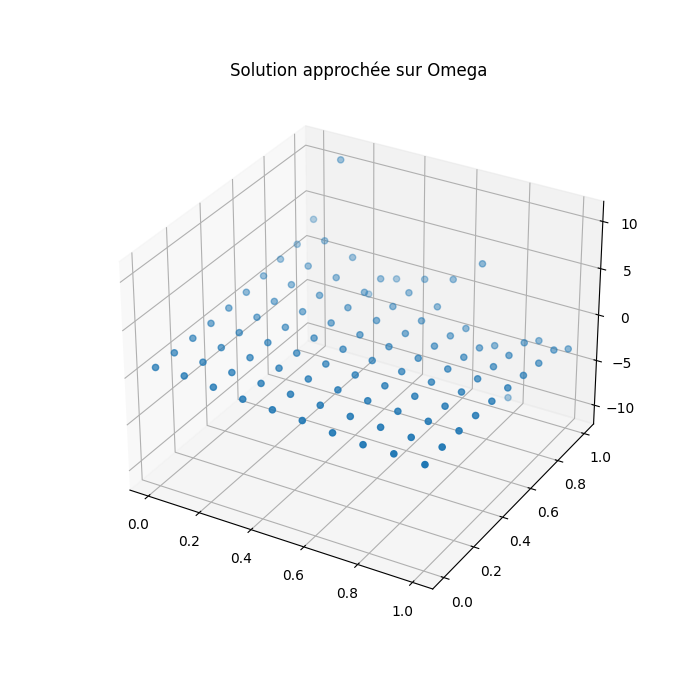
\includegraphics[width=7cm]{solcalc_omega.png}
  \label{fig/domaine}
  \caption{La solution approchée sur le maillage de $\Omega$}
\end{figure}

\vspace{1cm}
\newpage
\begin{figure}[h]
  \centering
  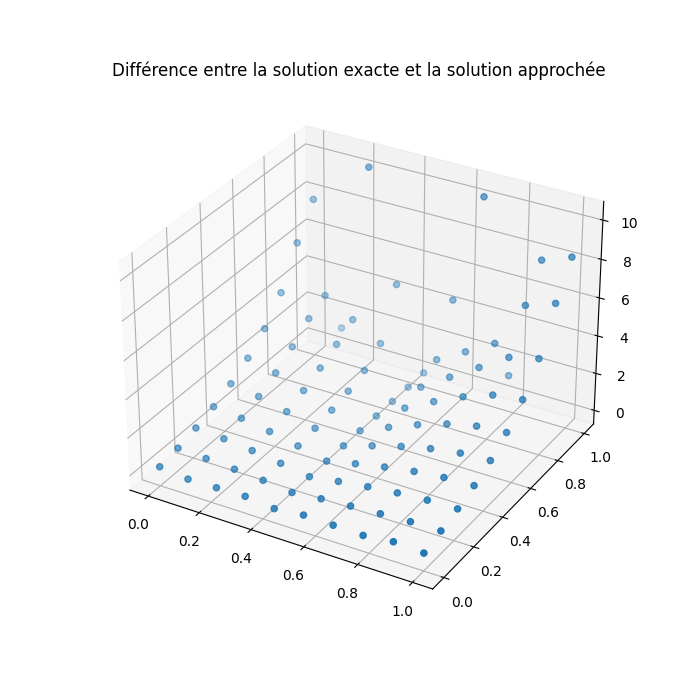
\includegraphics[width=10cm]{diff_omega.png}
  \label{fig/domaine}
  \caption{La différence absolue entre la solution exacte et la solution approchée sur le maillage de $\Omega$}
\end{figure}

\vspace{1cm}

On remarque, grâce à la dernière figure, que l'erreur est surtout faite sur le voisinage de $\Gamma_3$. Cela reflete l'approximation que l'on a prise sur la fonction $f_3$ par notre algorithme. Mais même en prenant en compte ces erreurs cela ne justifie pas la taille de ces erreurs ainsi cela renforce le faisceau presemption sur une approximation pas très bonne de $f_3$. En effet lorsque l'on injecte la fonction $f_3$ calculée à partir de la solution exacte on continue d'avoir une différence non négligeable au voisinage de $\Gamma_3$ :

\begin{figure}[h]
  \centering
  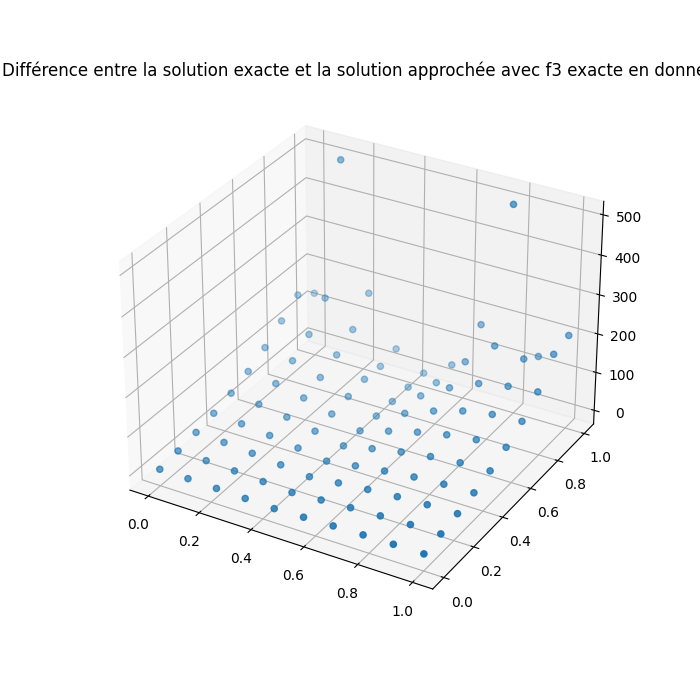
\includegraphics[width=7cm]{diff_omega_f3exacte.png}
  \label{fig/domaine}
  \caption{La différence absolue entre la solution exacte et la solution approchée avec $f_3$ en donnée}
\end{figure}

\vspace{1cm}




\newpage

Cela nous permet de déduire que l'erreur d'approximation provient de l'algorithme de calcul de la solution approchée plus que de l'approximation de la fonction $f_3$.

\section{Détermination de la frontière $\Gamma$}
Par définition si l'on choisit comme frontière $\Gamma$ paramètrisée par $x$, notée $\phi(x)$, on obtient pour $x\in [0,L]$:

\begin{equation}
    T_0(x) = u_ex(x,\phi(x))
\end{equation}

Ainsi on choisit $\phi$. Pour commencer on prend :
\begin{equation}
    \phi(x) = 0.2
\end{equation}

On obtient ainsi comme frontière $\Gamma$ :
\begin{figure}[h]
  \centering
  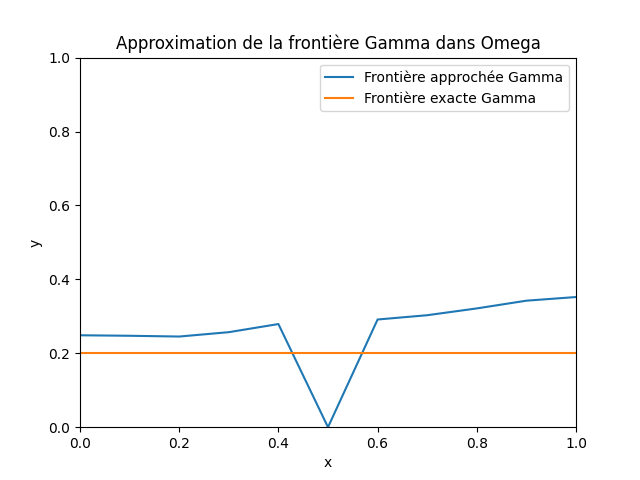
\includegraphics[width=7cm]{frontiere_Gamma_constante.png}
  \label{fig/domaine}
  \caption{Comparaison entre la frontière $\Gamma$ calculée et celle exacte.}
\end{figure}

\vspace{1cm}
On voit tout de suite un problème en $x = 0.5$. Celui-ci peut être contourné en prenant un maillage impair. Mais, par souci de transparence, on a ce problème lors de la recherche de la frontière $\Gamma$. Je pense que cela vient du fait que :
\begin{equation}
    u_ex(0.5,y) = 0
\end{equation}
Donc on n'a pas une unique solution au problème que l'on résout avec l'algorithme de Newton et ainsi on prend $y = 0$ comme solution pour le problème en $x = 0.5$. Cela explique le "creux" observé sur la représentation de $\Gamma$.


Maintenant prenons $\phi$ telle que :
\begin{equation}
    \phi(x) = 0.5x + 0.1
\end{equation}
Cela nous donne :
\begin{figure}[h]
  \centering
  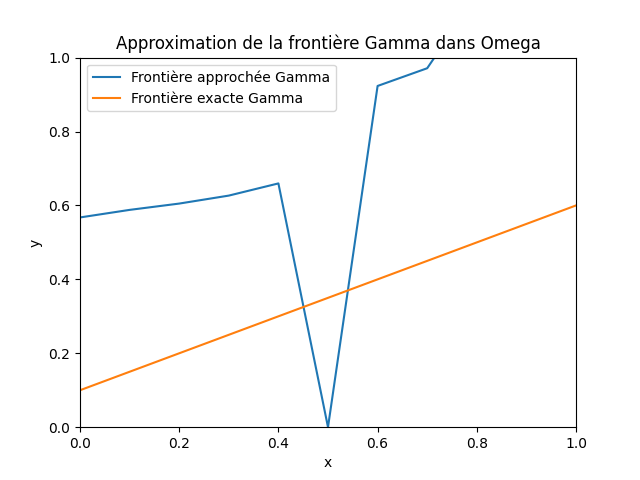
\includegraphics[width=7cm]{frontiere_Gamma_affine.png}
  \label{fig/domaine}
  \caption{Comparaison entre la frontière $\Gamma$ calculée et celle exacte.}
\end{figure}

\vspace{1cm}

On observe sur ce cas-ci un nouveau problème : la frontière $\Gamma$ est loin de la frontière exacte et sort du domaine $\Omega$.


Enfin on prend une frontière avec une forme sinusoïdale, c'est-à-dire :
\begin{equation}
    \phi(x) = 0.2sin(\pi x) + 0.5
\end{equation}
\begin{figure}[h]
    \centering
    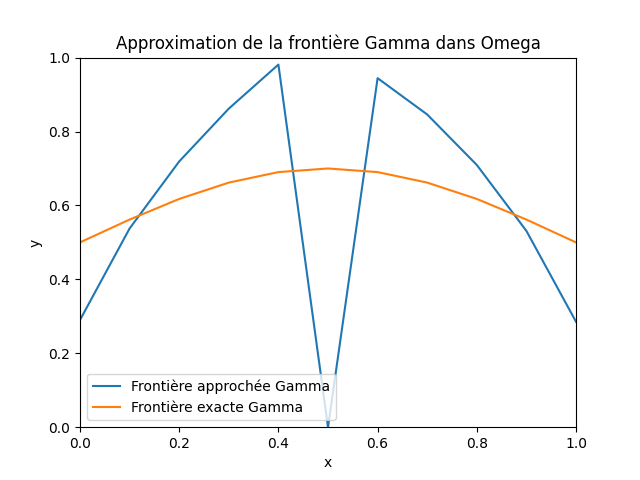
\includegraphics[width=7cm]{frontiere_Gamma_sinus.png}
    \caption{Comparaison entre la frontière $\Gamma$ calculée et celle exacte.}
    \label{fig:enter-label}
\end{figure}

Dans ce dernier cas l'approximation de la frontière $\Gamma$ reste très mauvaise malgré le fait que le comportement de la frontière exacte est suivi.
\section{Conclusion}
Pour conclure, l'implémentation de la méthode présentée ne semble pas optimale pour les problèmes étudiés. En effet, la solution approchée est particulièrement mauvaise au voisinage de $\Gamma_3$. De plus, la résolution de l'équation intégrale de Fredholm de seconde espèce n'est pas détaillée et cela ne permet pas de refaire les calculs pour s'approproprier la méthode.
Ces erreurs autour de $\Gamma_3$ se répercutent sur la détermination de la frontière $\Gamma$ du domaine qui ne semble pas très convaincante.


\section{Commentaire}
Le premier problème rencontré fut le passage de fonction en argument d'autre fonction, notamment pour construire la fonction de la méthode de quadrature de Gauss-Legendre, mais cela a été résolu grâce au passage d'un pointeur.


Ensuite je suis resté longtemps bloqué que le calcul de $\tilde{T}$ qui m'indiquait une très grande erreur $L^2(\Gamma_3)$ (i.e. de l'ordre de $10^3$). Après un intense déboggage et des échanges fructueux avec les membres de la classe, le problème se situait sur le fait que la série dans l'expression des coefficients de Fourrier $A_m$ et $B_m$ ne converge pas car en prenant plus des 1000 premiers termes on se retrouve avec une erreur de overflow du double précision. Cela provenait en partie de la solution exacte donnée à étudier qui ne vérifie pas toutes les conditions limites. 


Enfin lors du déboggage, je me suis documenté sur la façon la plus efficace de pouvoir effectuer cette tâche et en particulier la localisation de bug. Ainsi je change un booléen nommé $deboggage$ en pour avoir les logs de toutes les opérations intermédiaires et de la comparaison avec les données exactes.


Enfin, pour accélérer le processus de calcul on injecte l'expression analytique de $h$ dans $f_3$ ce qui permet de réduire une série à un unique terme par la relation d'orthogonalitée de $cos(\frac{m\pi x}{L})$.
\end{document}



